\documentclass[../main.tex]{subfiles}

\pagestyle{main}
\renewcommand{\chaptermark}[1]{\markboth{\chaptername\ \thechapter\ (#1)}{}}
\setcounter{chapter}{-1}

\begin{document}




\chapter{Course Prep}
\section{Chapter 1: Introduction to Inorganic Chemistry}
\emph{From \textcite{bib:MiesslerFischerTarr}.}
\subsection{Notes}
\begin{itemize}
    \item \marginnote{12/21:}\textbf{Inorganic chemistry}: The chemistry of everything that is not organic chemistry (the chemistry of hydrocarbon compounds and their derivatives).
    \item \textbf{Organometallic chemistry}: The chemistry of compounds containing metal-carbon bonds and the catalysis of many organic reactions.
    \item There is also both \textbf{bioinorganic chemistry} and \textbf{environmental chemistry} \parencite[1]{bib:MiesslerFischerTarr}, as well as \textbf{analytical chemistry}, \textbf{physical chemistry}, \textbf{petroleum chemistry}, \textbf{polymer chemistry} \parencite[4]{bib:MiesslerFischerTarr}.
    \begin{itemize}
        \item Note, though, that there are no strict dividing lines between subfields of chemistry nowadays, and most professionals work in multiple fields.
    \end{itemize}
    \item Single, double, and triple bonds (both metal-metal and metal-carbon bonds) are found in organic and inorganic chemistry.
    \item Quadruple bonds exist between metal atoms in some compounds.
    \begin{figure}[h!]
        \centering
        \begin{subfigure}[b]{0.3\linewidth}
            \centering
            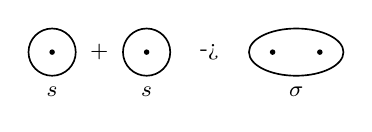
\begin{tikzpicture}
                \footnotesize
                \draw [semithick]
                    (0,0) circle (3mm)
                    (1.2,0) circle (3mm)
                    (3.1,0) ellipse (6mm and 3mm)
                ;

                \fill
                    (0,0) circle (1pt)
                    (1.2,0) circle (1pt)
                    (2.8,0) circle (1pt)
                    (3.4,0) circle (1pt)
                ;
                \node at (0.6,0) {$+$};
                \node at (2,0) {\ce{->}};

                \node at (0,-0.5) {$s$};
                \node at (1.2,-0.5) {$s$};
                \node at (3.1,-0.5) {$\sigma$};
            \end{tikzpicture}
            \caption{Sigma ($\sigma$) bond.}
            \label{fig:sigmaPiDeltaa}
        \end{subfigure}
        \begin{subfigure}[b]{0.3\linewidth}
            \centering
            \begin{tikzpicture}
                \footnotesize
                \filldraw [semithick,fill=gry]
                    (0,0.3) ellipse (3mm and 2mm)
                    (1.2,0.3) ellipse (3mm and 2mm)
                ;
                \draw [semithick]
                    (0,-0.3) ellipse (3mm and 2mm)
                    (1.2,-0.3) ellipse (3mm and 2mm)
                ;
                \draw [semithick,fill=gry] (2.6,0.05)
                    to[out=0,in=180,out looseness=0.5] (3.1,0.12)
                    to[out=0,in=180,in looseness=0.5] (3.6,0.05)
                    to[out=0,in=-90] (3.7,0.15)
                    to[out=90,in=0,out looseness=0.7,in looseness=0.8] (3.1,0.43)
                    to[out=180,in=90,out looseness=0.8,in looseness=0.7] (2.5,0.15)
                    to[out=-90,in=180] cycle
                ;
                \begin{scope}[yscale=-1]
                    \draw [semithick] (2.6,0.05)
                        to[out=0,in=180,out looseness=0.5] (3.1,0.12)
                        to[out=0,in=180,in looseness=0.5] (3.6,0.05)
                        to[out=0,in=-90] (3.7,0.15)
                        to[out=90,in=0,out looseness=0.7,in looseness=0.8] (3.1,0.43)
                        to[out=180,in=90,out looseness=0.8,in looseness=0.7] (2.5,0.15)
                        to[out=-90,in=180] cycle
                    ;
                \end{scope}

                \fill
                    (0,0) circle (1pt)
                    (1.2,0) circle (1pt)
                    (2.8,0) circle (1pt)
                    (3.4,0) circle (1pt)
                ;
                \node at (0.6,0) {$+$};
                \node at (2,0) {\ce{->}};

                \node at (0,-0.7) {$p$};
                \node at (1.2,-0.7) {$p$};
                \node at (3.1,-0.7) {$\pi$};
            \end{tikzpicture}
            \caption{Pi ($\pi$) bond.}
            \label{fig:sigmaPiDeltab}
        \end{subfigure}
        \begin{subfigure}[b]{0.3\linewidth}
            \centering
            \begin{tikzpicture}
                \footnotesize
                \draw [semithick]
                    (0.08,0.01) ellipse (3mm and 2mm)
                    (1.28,0.01) ellipse (3mm and 2mm)
                ;
                \filldraw [semithick,fill=gry]
                    (0,0.3) ellipse (3mm and 2mm)
                    (1.2,0.3) ellipse (3mm and 2mm)
                    (0,-0.3) ellipse (3mm and 2mm)
                    (1.2,-0.3) ellipse (3mm and 2mm)
                ;
                \filldraw [semithick,fill=white]
                    (-0.08,-0.01) ellipse (3mm and 2mm)
                    (1.12,-0.01) ellipse (3mm and 2mm)
                ;
                \draw [semithick]
                    (3.18,0.01) ellipse (6mm and 2mm)
                ;
                \draw [semithick,fill=gry] (2.6,0.05)
                    to[out=0,in=180,out looseness=0.5] (3.1,0.12)
                    to[out=0,in=180,in looseness=0.5] (3.6,0.05)
                    to[out=0,in=-90] (3.7,0.15)
                    to[out=90,in=0,out looseness=0.7,in looseness=0.8] (3.1,0.43)
                    to[out=180,in=90,out looseness=0.8,in looseness=0.7] (2.5,0.15)
                    to[out=-90,in=180] cycle
                ;
                \begin{scope}[yscale=-1]
                    \draw [semithick,fill=gry] (2.6,0.05)
                        to[out=0,in=180,out looseness=0.5] (3.1,0.12)
                        to[out=0,in=180,in looseness=0.5] (3.6,0.05)
                        to[out=0,in=-90] (3.7,0.15)
                        to[out=90,in=0,out looseness=0.7,in looseness=0.8] (3.1,0.43)
                        to[out=180,in=90,out looseness=0.8,in looseness=0.7] (2.5,0.15)
                        to[out=-90,in=180] cycle
                    ;
                \end{scope}
                \filldraw [semithick,fill=white]
                    (3.02,-0.01) ellipse (6mm and 2mm)
                ;

                \fill
                    (0,0) circle (1pt)
                    (1.2,0) circle (1pt)
                    (2.8,0) circle (1pt)
                    (3.4,0) circle (1pt)
                ;
                \node at (0.6,0) {$+$};
                \node at (2,0) {\ce{->}};

                \node at (0,-0.7) {$d$};
                \node at (1.2,-0.7) {$d$};
                \node at (3.1,-0.7) {$\delta$};
            \end{tikzpicture}
            \caption{Delta ($\delta$) bond.}
            \label{fig:sigmaPiDeltac}
        \end{subfigure}
        \caption{Examples of bonding interactions.}
        \label{fig:sigmaPiDelta}
    \end{figure}
    \begin{itemize}
        \item No such bonds exist between carbon atoms because two carbon atoms max out at a triple bond.
        \item Quadruple bonds possess one sigma bond, two pi bonds, and one delta ($\delta$) bond.
        \item The delta bond is only possible with metal atoms because these atoms possess energetically accessible $d$ orbitals.
    \end{itemize}
    \item Quintuple bonds between transition metals have been reported, but scientists have not yet reached a consensus on to what extent these exist.
    \begin{figure}[h!]
        \centering
        \footnotesize
        \chemfig[atom sep=2em,fixed length=true,bond offset=3pt,cram width=3pt]{H-[:-25,,,,dash pattern=on 2pt off 2pt]B(<[:-155]H)(-[7]H?)-[1]H-[7]B?(-[:25,,,,dash pattern=on 2pt off 2pt]H)<[:-25]H}
        \hspace{5em}
        \chemfig[atom sep=2em,fixed length=true,bond offset=3pt,cram width=3pt]{H_3C-[:-25,,,,dash pattern=on 2pt off 2pt]Al(<[:-155]H_3C)(-[7]\chembelow{C}{\hspace{4pt}H_3}?)-[1]\chemabove{C}{\hspace{4pt}H_3}-[7]Al?(-[:25,,,,dash pattern=on 2pt off 2pt]CH_3)<[:-25]CH_3}
        \caption{Inorganic compounds containing bridging hydrogens and alkyl groups.}
        \label{fig:bridgingH-CH3}
    \end{figure}
    \item Hydrogen atoms and alkyl groups can act as bridges in inorganic chemistry, excessively disobeying the octet rule (see Figure \ref{fig:bridgingH-CH3}).
    \item \textbf{Coordination number}: The number of other atoms, molecules, or ions to which an atom is bonded.
    \item "Numerous inorganic compounds have central atoms with coordination numbers of five, six, seven, and higher" \parencite[2]{bib:MiesslerFischerTarr}.
    \begin{itemize}
        \item The most common coordination geometry for transition metals is octahedral.
    \end{itemize}
    \item 4-coordinate carbon is almost always tetrahedral. 4-coordinate metals and nonmetals can be either tetrahedral or square planar.
    \item \textbf{Coordination complex}: A compound with a metal as the central atom or ion and some number of \textbf{ligands} bonded to it.
    \item \textbf{Ligand}: An anion or neutral molecule bonded to a central atom (frequently through \ce{N}, \ce{O}, or \ce{S}).
    \item \textbf{Organometallic complex}: A coordination complex where carbon (potentially bonded to other things) is one of the ligands.
    \begin{figure}[h!]
        \centering
        \footnotesize
        \chemfig[atom sep=5em]{P?[1]-[:53]P(-[6]P?[1]?[3])-[:-53]P?[3]?[1,1,{dash pattern=on 2pt off 2pt}]}
        \caption{Tetrahedral geometry without a central atom.}
        \label{fig:tetrahedralNoCentral}
    \end{figure}
    \item There are multiple kinds of tetrahedral structures. There is the standard arrangement seen in molecules such as methane, but there is also a form that lacks a central atom, as in elemental phosphorous \ce{P4} (see Figure \ref{fig:tetrahedralNoCentral}).
    \begin{itemize}
        \item Other atoms such as boron and carbon also form units that surround a central cavity (e.g., icosahedral \ce{B12} and buckyballs \ce{C60}).
    \end{itemize}
    \item Aromatic rings can bond to metals using all of their pi orbitals. This results in a metal suspended above the ring's center.
    \item \textbf{Cluster compound}: A compound where "a carbon atom is at the center of a polyhedron of metal atoms" \parencite[3]{bib:MiesslerFischerTarr}.
    \begin{itemize}
        \item There exist examples of carbon surrounded by five, six, or more metal atoms\footnote{This provides a challenge to theoretical inorganic chemists.}.
    \end{itemize}
    \item Many new forms of elemental carbon have been discovered since the mid-1980s, notably including fullerenes (such as buckminsterfullerene, or buckyballs), carbon nanotubes, graphene, and polyyne wires.
    \item \textcite{bib:MiesslerFischerTarr} give a brief history of inorganic chemistry for context.
    \begin{itemize}
        \item Be aware of \textbf{crystal field theory} and \textbf{ligand field theory}.
    \end{itemize}
\end{itemize}
\newpage



\section{Chapter 2: Atomic Structure}
\emph{From \textcite{bib:MiesslerFischerTarr}.}
\subsection{Notes}
\begin{itemize}
    \item \marginnote{12/22:}\textbf{Coinage metals}: Copper, silver, and gold, i.e., the transition metals in IUPAC Group 11.
    \item \textbf{Chalcogens}: Oxygen, sulfur, selenium, tellurium, and polonium, i.e., the nonmetals in Group 16.
    \item The energies of visible light emitted by the hydrogen atom are given by\footnote{Refer to \textcite{bib:APChemNotes}, specifically Figure 7.6 and the accompanying discussion.}
    \begin{equation*}
        E = R_H\left( \frac{1}{2^2}-\frac{1}{n_h^2} \right)
    \end{equation*}
    where $n_h$ is an integer greater than 2 and $R_H$ is the Rydberg constant for hydrogen (\ce{H}).
    \begin{itemize}
        \item Note that $
            R_H = \SI{1.097e7}{\per\meter}
            = \SI{2.179e-18}{\joule}
            = \SI{13.61}{eV}
        $.
        \item This equation was first discovered by Johann Balmer in 1885.
        \item Infrared and ultraviolet emissions can be described by replacing $2^2$ with integers $n_l^2$ in the above equation on the condition that $n_l<n_h$\footnote{$n_l$ denotes the \underline{l}ower final energy level while $n_h$ denotes the \underline{h}igher initial energy level.}.
    \end{itemize}
    \item The energy of the light emitted is related to its wavelength, frequency, and wavenumber by the equations
    \begin{equation*}
        E = h\nu = \frac{hc}{\lambda} = hc\bar{\nu}
    \end{equation*}
    where $h$ is Planck's constant ($\SI{6.626e-34}{\joule\second}$), $c$ is the speed of light ($\SI{2.998e8}{\meter\per\second}$), and $\nu$, $\lambda$, and $\bar{\nu}$ are the frequency, wavelength, and \textbf{wavenumber}, respectively, of the light.
    \item \textbf{Wavenumber}: The number of waves that exist between two points along the light's path a given distance apart. \emph{Measured in} waves per centimeter (SI: $\si{\per\centi\meter}$).
    \begin{itemize}
        \item Wavenumber is proportional to energy. This is why $\si{\per\meter}$ or $\si{\per\centi\meter}$ can be used as an energy unit.
    \end{itemize}
    \item \textbf{Principal quantum number}: One of the quantities $n$ in Balmer's equation.
    \item Bohr's atomic theory first explained the phenomenon of Balmer's equation, positing that "electrons may absorb light of certain specific energies and be excited to orbits of higher energy; they may also emit light of specific energies and fall to orbits of lower energy" \parencite[11-12]{bib:MiesslerFischerTarr}.
    \begin{itemize}
        \item Bohr rewrote the Rydberg constant in terms of other quantities:
        \begin{equation*}
            R = \frac{2\pi^2\mu Z^2e^4}{(4\pi\varepsilon_0)^2h^2}
        \end{equation*}
        where\dots
        \begin{itemize}
            \item $\mu$ is the reduced mass of the electron/nucleus combination $\frac{1}{\mu}=\frac{1}{m_e}+\frac{1}{m_\text{nucleus}}$, where $m_e=\SI{9.11e-31}{\kilo\gram}$ is the mass of the electron and $m_\text{nucleus}$ is the mass of the nucleus.
            \item $Z$ is the nuclear charge.
            \item $e=\SI{1.602e-19}{\coulomb}$ is the charge of the electron.
            \item $h$ is Planck's constant.
            \item $4\pi\varepsilon_0$ is the permittivity of a vacuum.
        \end{itemize}
        \item Importantly, note that the Rydberg constant for hydrogen $R_H$ is not universal, and changes for the atom at hand based on factors like the mass of the nucleus.
    \end{itemize}
    \begin{figure}[h!]
        \centering
        \begin{tikzpicture}[yscale=17]
            \footnotesize
            \foreach \y in {1,...,6} {
                \draw [thick] (0,{-1/(\y*\y)}) -- ++(10.5,0) node[right]{$\y$};
            }
            \foreach \y in {7,...,11} {
                \draw [thick] (0,{-1/(\y*\y)}) -- ++(10.5,0);
            }
            \fill (0,{-1/121}) rectangle (10.5,0) node[right]{$\infty$};
    
            \foreach \x in {1,...,5} {
                \draw [semithick,grx,-latex] ({0.05+\x*0.25},{-1/(\x+1)^2}) -- ({0.05+\x*0.25},-1);
            }
            \node [anchor=west,text width=1cm,align=center] at (1.4,{(-1/1-1/4)/2}) {Lyman series (UV)};
            \foreach \x in {2,...,5} {
                \draw [semithick,grx,-latex] ({3.05+\x*0.25},{-1/(\x+1)^2}) -- ({3.05+\x*0.25},{-1/4});
            }
            \node [anchor=west,text width=4cm] at (4.4,{(-1/4-1/9)/2}) {Balmer series\\ (visible transitions shown)};
            \foreach \x in {3,...,5} {
                \draw [semithick,grx,-latex] ({6.05+\x*0.25},{-1/(\x+1)^2}) -- ({6.05+\x*0.25},{-1/9});
            }
            \node [anchor=west] at (7.4,{(-1/9-1/16)/2}) {Paschen series (IR)};
        \end{tikzpicture}
        \caption{Hydrogen atom energy levels.}
        \label{fig:energyLevelH}
    \end{figure}
    \item \textbf{Balmer series}: The four main electron transitions in hydrogen that release electromagnetic radiation in the visible spectrum.
    \item \textbf{Lyman series}: The five main electron transitions in hydrogen that release electromagnetic radiation in the ultraviolet spectrum.
    \item \textbf{Paschen series}: The three main electron transitions in hydrogen that release electromagnetic radiation in the infrared spectrum.
    \item "The inverse square dependence of energy on $n$ results in energy levels that are far apart in energy at small $n$ and become much closer in energy at larger $n$" \parencite[12]{bib:MiesslerFischerTarr}
    \begin{itemize}
        \item Individual electrons can have more energy than they would possess in the infinite energy level, but at and above this point, the nucleus and electron are considered to be separate entities.
    \end{itemize}
    \item \textbf{Heisenberg's uncertainty principle}: "There is a relationship between the inherent uncertainties in the location and momentum of an electron" \parencite[14]{bib:MiesslerFischerTarr}.
    \begin{equation*}
        \Delta x\, \Delta p_x \geq \frac{h}{4\pi}
    \end{equation*}
    \begin{itemize}
        \item The above equation describes the $x$-component of the uncertainty, where $\Delta x$ is the uncertainty in the position of the electron and $\Delta p_x$ is the uncertainty in the momentum of the electron in the $x$-direction.
    \end{itemize}
    \item Because of the uncertainty principle, we cannot treat electrons as particles with precisely described motion; instead, we must describe them in \textbf{orbitals}.
    \item \textbf{Orbital}: A region that describes the probable locations of an electron.
    \item \textbf{Electron density}: "The probability of finding the electron at a particular point in space" \parencite[14]{bib:MiesslerFischerTarr}.
    \begin{itemize}
        \item This can be calculated in principle.
    \end{itemize}
    \item Schr\"{o}dinger and Heisenberg published (in 1926 and 1927, respectively) papers on atomic wave mechanics. Although they used very different mathematical techniques, their theories can be shown to be equivalent. However, we will introduce Schr\"{o}dinger's more commonly used differential equations.
    \item "The Schr\"{o}dinger equation describes the wave properties of an electron in terms of its position, mass, total energy, and potential energy" \parencite[14]{bib:MiesslerFischerTarr}.
    \begin{equation*}
        H\Psi = E\Psi
    \end{equation*}
    \begin{itemize}
        \item In its simplest form, it is given by the above, where $H$ is the \textbf{Hamiltonian operator}, $E$ is the energy of the electron, and $\Psi$ is the \textbf{wave function}.
    \end{itemize}
    \item \textbf{Wave function}: A function that describes an electron wave in space, i.e., an atomic orbital.
    \item Energy values are another way of describing the quantization introduced with the Bohr model --- different orbitals, characterized by different wave functions, each have characteristic energies.
    \item \textbf{Operator}: "An instruction or set of instructions that states what to do with the function that follows it" \parencite[14]{bib:MiesslerFischerTarr}.
    \item \textbf{Hamiltonian operator}: An operator including derivatives that transforms the wave function into a constant (the energy) times $\Psi$. \emph{Also known as} $\bm{\hat{H}}$.
    \begin{equation*}
        H = \frac{-h^2}{8\pi^2m}\left( \pdv[2]{x}+\pdv[2]{y}+\pdv[2]{z} \right)-\frac{Ze^2}{4\pi\varepsilon_0\sqrt{x^2+y^2+z^2}}
    \end{equation*}
    \begin{itemize}
        \item In the form used for calculating the energy levels of one-electron systems, it is given by the above, where\dots
        \begin{itemize}
            \item $h$ is Planck's constant.
            \item $m$ is the mass of the electron.
            \item $e$ is the charge of the electron.
            \item $\sqrt{x^2+y^2+z^2}=r$ is the distance from the nucleus.
            \item $Z$ is the charge of the nucleus.
            \item $4\pi\varepsilon_0$ is the permittivity of a vacuum.
        \end{itemize}
        \item The first part describes the kinetic energy of the electron, its energy of motion.
        \item The second part describes the potential energy of the electron, the result of the electrostatic attraction between it and the nucleus. It is commonly designated as $V(x,y,z)$.
    \end{itemize}
    \item "Because $n$ varies from 1 to $\infty$, and every atomic orbital is described by a unique $\Psi$, there is no limit to the number of solutions of the Schr\"{o}dinger equation for an atom. Each $\Psi$ describes the wave properties of a given electron in a particular orbital" \parencite[15]{bib:MiesslerFischerTarr}.
    \item Electron density is proportional to $\Psi^2$.
    \item Necessary conditions for a physically realistic solution for $\Psi$:
    \begin{enumerate}
        \item $\Psi$ must be single-valued: There cannot be two probabilities for an electron at any position in space.
        \item $\Psi$ and its first derivatives must be continuous: The probability must be defined at all positions in space and cannot change abruptly from one point to the next.
        \item $\Psi$ must approach zero as $r\to\infty$: For large distances from the nucleus, the probability must grow smaller and smaller (the atom must be finite).
        \item The integral
        \begin{equation*}
            \int\limits_\text{all space}\Psi_A{\Psi_A}^*\dd{\tau} = 1
        \end{equation*}
        The total probability of an electron being somewhere in space must be 1. Applying this stipulation is called \textbf{normalizing} the wave function\footnote{${\Psi_A}^*$ denotes the complex conjugate of $\Psi_A$. This is necessary because wave functions may have imaginary values. However, in many cases, the wave functions are real and the integrand reduces to $\Psi_A^2$.}.
        \item The integral
        \begin{equation*}
            \int\limits_\text{all space}\Psi_A{\Psi_B}^*\dd{\tau} = 0
        \end{equation*}
        $\Psi_A$ and $\Psi_B$ are different orbitals within the same atom, and this stipulation reflects the fact that all orbitals in the same atom must be \textbf{orthogonal} to each other.
    \end{enumerate}
\end{itemize}


\subsection{Problems}
\begin{enumerate}[label={\textbf{2.\arabic*}}]
    \setcounter{enumi}{7}
    \item \marginnote{9/13:}The details of several steps in the particle-in-a-box model in this chapter have been omitted. Work out the details of the following steps:
    \begin{enumerate}[label={\textbf{\alph*.}}]
        \item Show that if $\Psi=A\sin rx+B\cos sx$ ($A$, $B$, $r$, and $s$ are constants) is a solution to the wave equation for the one-dimensional box, then
        \begin{equation*}
            r = s = \sqrt{2mE}\left( \frac{2\pi}{h} \right)
        \end{equation*}
        \begin{proof}[Solution]
            \allowdisplaybreaks
            \begin{align*}
                \frac{-h^2}{8\pi^2m}\cdot\pdv[2]{\Psi(x)}{x} &= E\Psi(x)\\
                \frac{-h^2}{8\pi^2m}\cdot\pdv[2]{x}\left( A\sin rx+B\cos sx \right) &= E(A\sin rx+B\cos sx)\\
                \frac{-h^2}{8\pi^2m}\cdot\pdv{x}\left( Ar\cos rx-Bs\sin sx \right) &= E(A\sin rx+B\cos sx)\\
                \frac{-h^2}{8\pi^2m}\cdot\left( -Ar^2\sin rx-Bs^2\cos sx \right) &= E(A\sin rx+B\cos sx)\\
                \frac{Ar^2h^2}{8\pi^2m}\sin rx+\frac{Bs^2h^2}{8\pi^2m}\cos sx &= AE\sin rx+BE\cos sx\\
                0 &= \left( \frac{Ar^2h^2}{8\pi^2m}-AE \right)\sin rx+\left( \frac{Bs^2h^2}{8\pi^2m}-BE \right)\cos sx
                \intertext{Choose $x=0$.}
                &= \frac{Bs^2h^2}{8\pi^2m}-BE\\
                E &= \frac{s^2h^2}{8\pi^2m}\\
                \frac{8\pi^2mE}{h^2} &= s^2\\
                s &= \sqrt{\frac{8\pi^2mE}{h^2}}\\
                \Aboxed{s &= \sqrt{2mE}\frac{2\pi}{h}}
                \intertext{With this result \dots}
                0 &= \left( \frac{Ar^2h^2}{8\pi^2m}-AE \right)\sin rx+\left( \frac{Bs^2h^2}{8\pi^2m}-BE \right)\cos sx\\
                &= \left( \frac{Ar^2h^2}{8\pi^2m}-AE \right)\sin rx+\left( B\left( \frac{s^2h^2}{8\pi^2m} \right)-BE \right)\cos sx\\
                &= \left( \frac{Ar^2h^2}{8\pi^2m}-AE \right)\sin rx+\left( BE-BE \right)\cos sx\\
                &= \left( \frac{Ar^2h^2}{8\pi^2m}-AE \right)\sin rx\\
                \intertext{Choose $x=\frac{\pi}{2r}$.}
                &= \frac{Ar^2h^2}{8\pi^2m}-AE\\
                \Aboxed{r &= \sqrt{2mE}\frac{2\pi}{h}}
            \end{align*}
        \end{proof}
        \setcounter{enumii}{3}
        \item Show that substituting the value of $r$ given in part c into $\Psi=A\sin rx$ and applying the normalizing requirement gives $A=\sqrt{2/a}$.
        \begin{proof}[Solution]
            \begin{align*}
                1 &= \int_\text{all space}\Psi\Psi^*\dd{\tau}\\
                &= \int_0^a \left( A\sin\frac{n\pi x}{a} \right)\left( A\sin\frac{n\pi x}{a} \right)\dd{x}\\
                &= \int_0^a A^2\sin^2\frac{n\pi x}{a}\dd{x}
                \intertext{Use $\sin^2u=\frac{1-\cos2u}{2}$.}
                &= A^2\int_0^a \frac{1-\cos\frac{2n\pi x}{a}}{2}\dd{x}\\
                &= \frac{A^2}{2}\left( \int_0^a \dd{x}-\int_0^a \cos\frac{2n\pi x}{a}\dd{x} \right)\\
                &= \frac{A^2}{2}\left( [x]_0^a-\left[ \frac{a}{2n\pi}\sin\frac{2n\pi x}{a} \right]_0^a \right)\\
                &= \frac{A^2}{2}\left( (a-0)-\left( \frac{a}{2n\pi}\sin 2n\pi-\frac{a}{2n\pi}\sin 0 \right) \right)\\
                &= \frac{A^2}{2}\left( a-\left( \frac{a}{2n\pi}\sin 2n\pi \right) \right)
                \intertext{Since $n$ is an integer, $\sin 2n\pi=0$.}
                &= \frac{aA^2}{2}\\
                \frac{2}{a} &= A^2\\
                \Aboxed{A &= \sqrt{\frac{2}{a}}}
            \end{align*}
        \end{proof}
    \end{enumerate}
\end{enumerate}




\end{document}